% Figure 13 supplementary-material insert for the v2.1.0 development gate.
% The published v2.0.0 supplement and accepted source-v1 paper remain frozen.

\subsection{Stylised facts under operational and calendar observation}
\label{app:stylised-facts-recovery}

Figure~\ref{fig:stylised-facts-recovery} retains the panel hierarchy of Bauer
et al. as a structural reference while changing the estimands to match the
current theory and available provenance.  The earlier figure compares
empirical data with a calibrated non-uniform-time legacy implementation.  The
present figure compares one current-model ensemble before and after a separate
previous-refresh observation map.  The operational model evolves on a fixed
grid; calendar non-uniformity enters only through subordination.  Log-mid
displacement is reported relative to the translation-invariant zero origin,
so its level cannot be compared with the arbitrary price levels in the legacy
figure.

The production event process uses irregular background market-order arrivals
at the declared mean rate.  Event quantity is fixed from the full-experiment
event/background displacement scale rather than from the earlier impact-test
quantity.  No smoothing, path selection or parameter refit is used.  The
accepted ensemble contains 16 paths and 5,600 operational steps per path; the
extension from 2,800 steps was required to obtain at least 25 operational
observations beyond $|z|>3$ under the registered tail gate.

The distinction between the two rows explains the principal morphological
difference.  The operational row has no zero-return atom and is close to
Gaussian for the registered baseline.  The calendar row holds the last
available value between refreshes, creating 60.49\% zero five-second
increments, a central density spike, an extended QQ plateau and larger
standardised tails.  These are observation-clock effects; they do not imply
that the underlying operational path has changed.

The baseline uses ordinary operational order $\alpha_u=1$, zero cancellation
and a Poisson refresh clock.  It therefore does not test fractional
operational memory or non-Markovian calendar waiting times.  Those mechanisms
remain distinct in the Angstmann--Gebbie formulation and require their own
registered numerical controls before use.  Signed-order-flow persistence is
imposed by the declared finite-persistence aggressor-sign input and is not an
endogenous model result.

\begin{figure}[p]
\centering
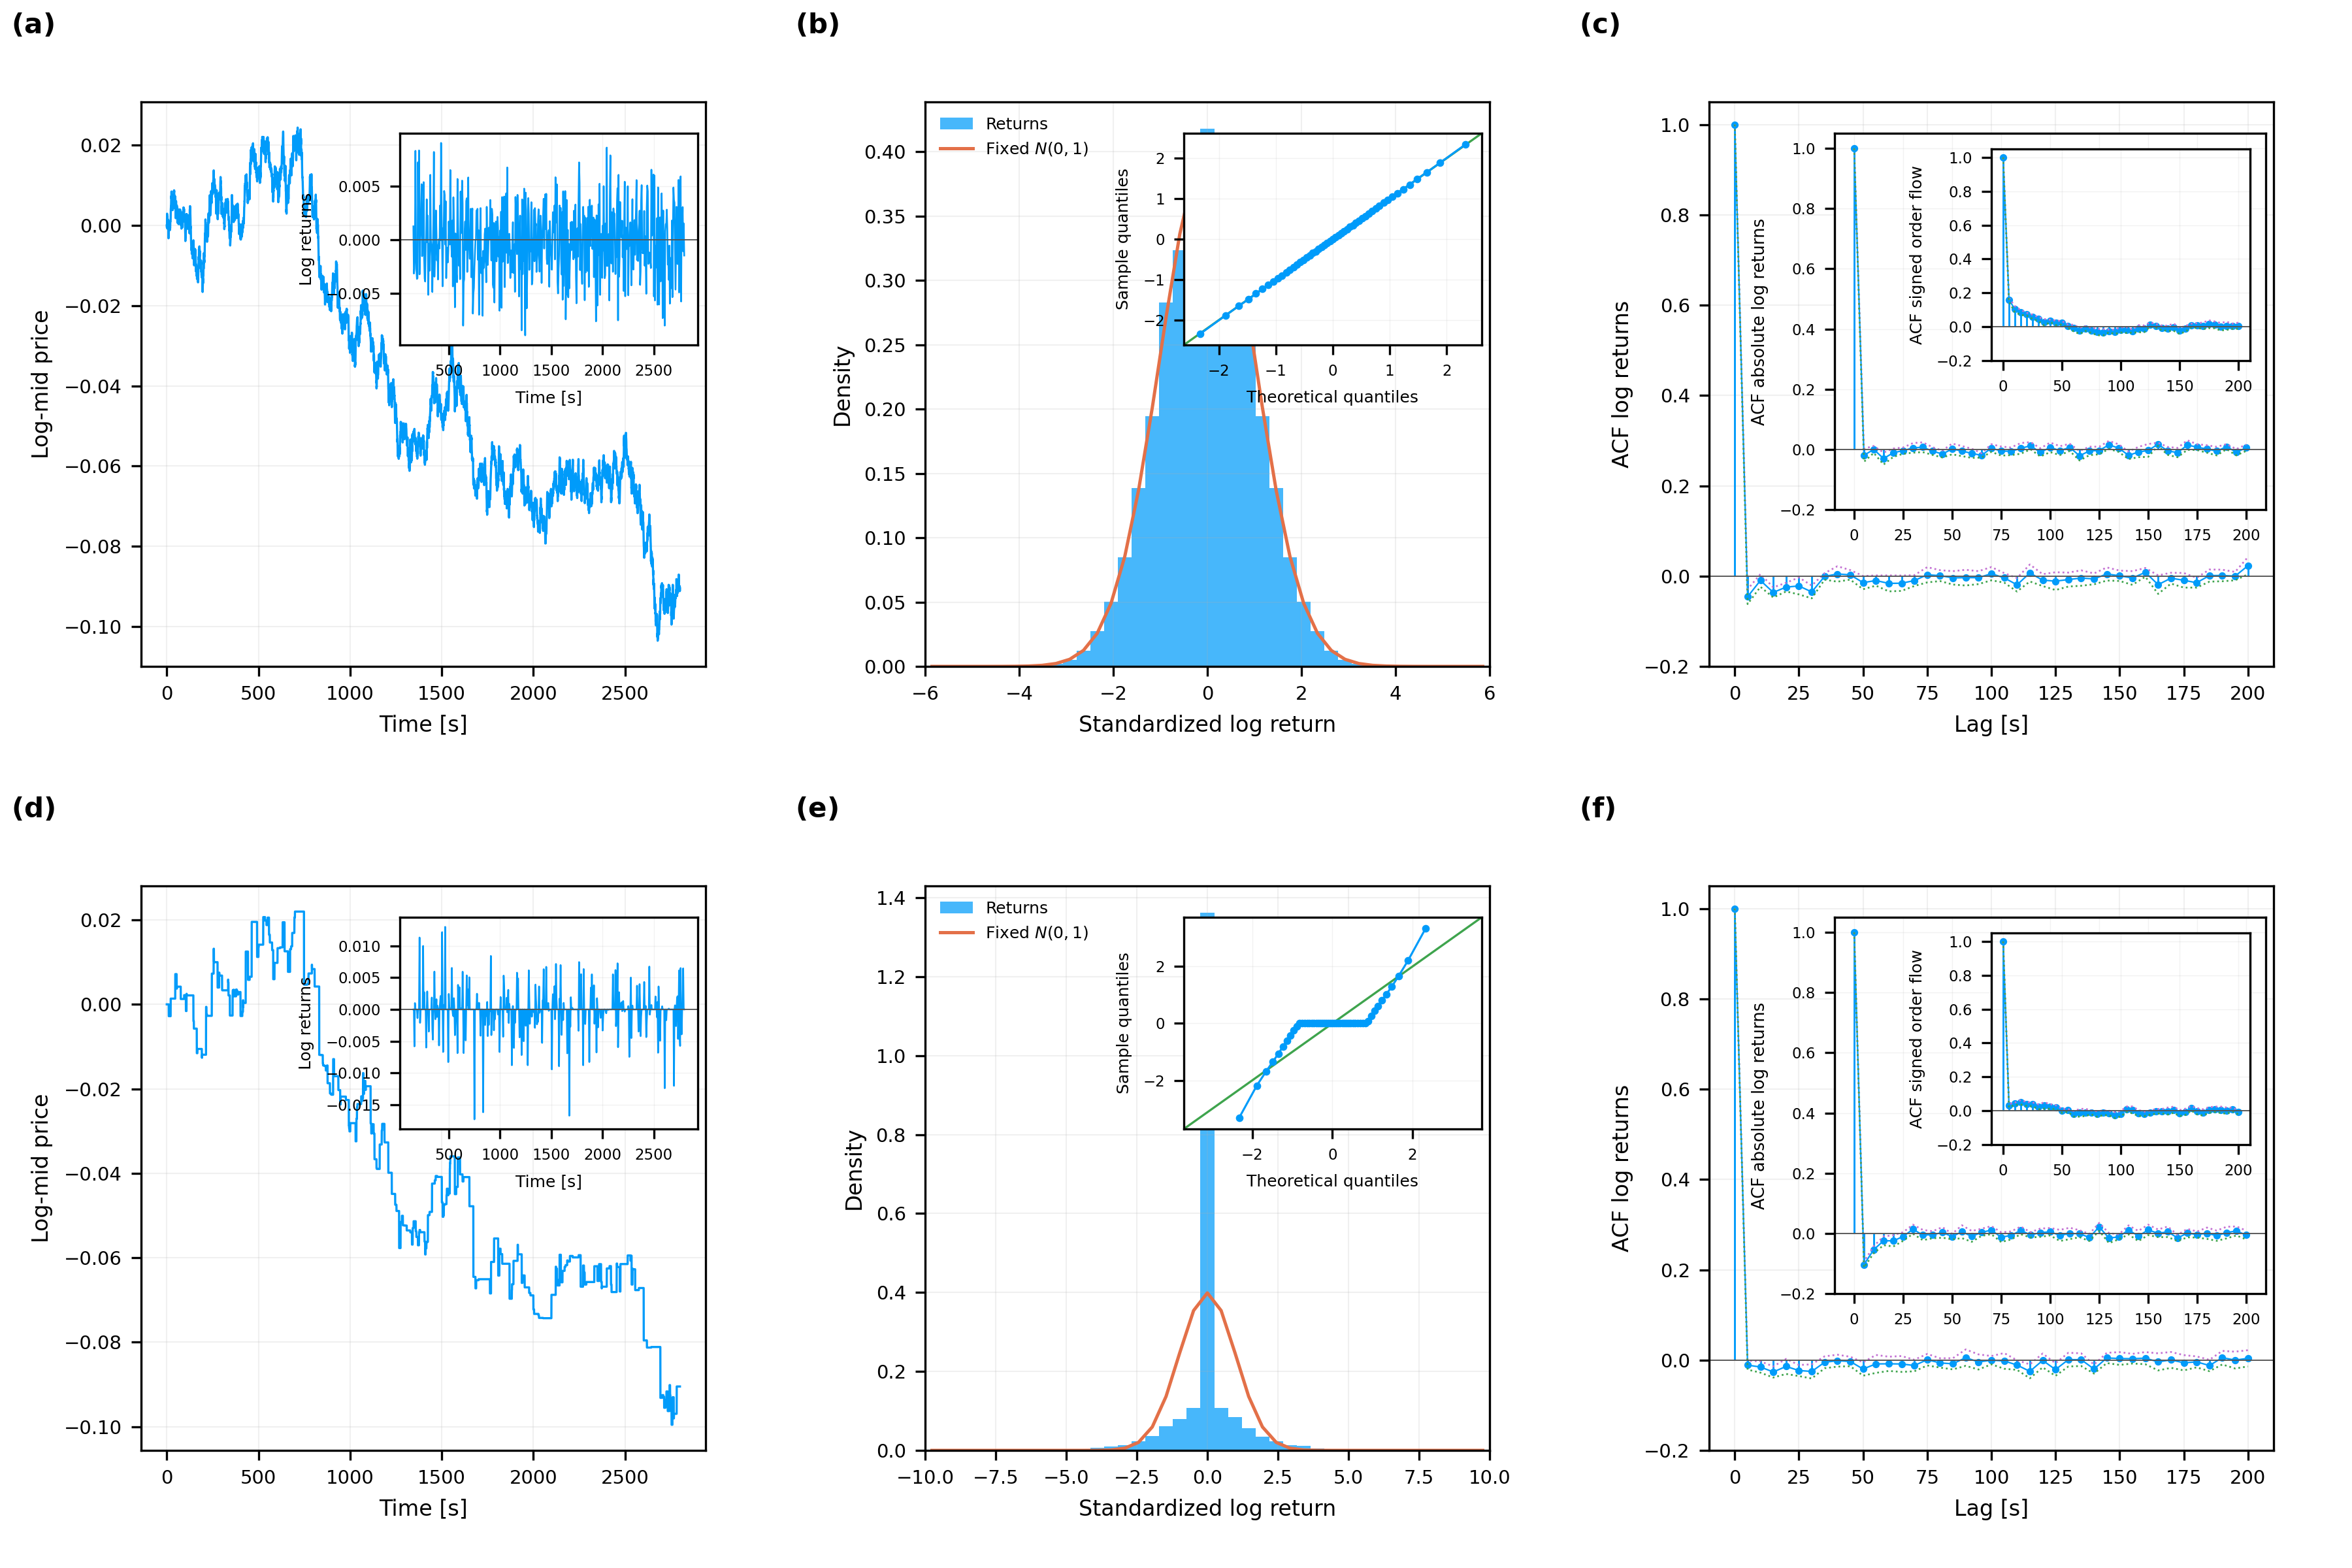
\includegraphics[width=\textwidth]{figures/figure-13-stylised-facts-recovery-v2.png}
\caption{\textbf{Current-model stylised facts under operational and calendar
observation.} Panels (a)--(c) use five-second increments on the uniform
operational grid; panels (d)--(f) use previous-refresh calendar observations
of the same simulated paths. Panels (a) and (d) show the Book 1 log-mid
displacement for the registered representative path, with unstandardised log
returns inset. Panels (b) and (e) show pooled standardised-return densities
with the fixed standard-normal reference and normal-QQ insets. Panels (c) and
(f) show ensemble log-return ACFs, with absolute-log-return and declared-
aggressor signed-order-flow ACFs nested in the same order as Bauer et al. Blue
curves are model estimates; orange is the standard-normal reference, green is
the QQ identity or lower pointwise uncertainty curve, and magenta is the upper
pointwise uncertainty curve. The fixed-grid implementation uses $\alpha_u=1$
and zero cancellation. The calendar path is stepwise because previous-refresh
observation holds the last operational log-mid value between asynchronous
refreshes. This creates a central zero-return mass and stronger calendar-time
tail curvature without changing the underlying operational path. Unlike Bauer
et al. Figure 3, the rows are an operational/calendar comparison rather than
empirical/calibrated data; no empirical row, legacy fractional recurrence or
absolute price-level claim is made. Signed-order-flow persistence is imposed
by the declared finite-persistence input and is not an endogenous result.}
\label{fig:stylised-facts-recovery}
\end{figure}
